\chapter{Model Transformation}
\label{sec:user_trafo}

The core of the Visual Service Design Tool clearly is the transformation to
executable code.  Currently, both the transformations to BPEL and to JIAC agent
services can conveniently be used in practice.

For directions on how to invoke the transformation please refer to
Section~\ref{sec:user_tut_export}.


%%%%%%%%%%%%%%%%%%%%%%%%%%%%%%%%%%%%%%%%%%%%%%%%%%%%%%%%%%%%%%%%%%%%%%%%%%%%%%%%
%%  Understanding the Transformation Framework                                %%
%%%%%%%%%%%%%%%%%%%%%%%%%%%%%%%%%%%%%%%%%%%%%%%%%%%%%%%%%%%%%%%%%%%%%%%%%%%%%%%%

\section{Understanding the Transformation Framework}
\label{sec:user_trafo_intro}

This section will provide a brief introduction in the basics of the transformation
framework.  The transformation framework has been designed from the very beginning
to be as \emph{extensible} and \emph{reusable} as possible.  For that purpose the
process of transformation has been subdivided into several stages, which are
sequentially applied to the input model:
\begin{enumerate}
	\item In the \emph{Validation} stage, all identifiers are validated to contain
	only characters that are legal with respect to the given target language.
	Further, the validation will check if each element needed is in place and
	provide clear error messages in case something is missing.

	\item The intent of the \emph{Normalization} stage is to put the process
	diagram in a uniform form, and to transform it to a semantically equivalent
	representation of the diagram following more strict constraints than those
	given in the BPMN specification.

	\item In the \emph{Structure Mapping} stage, the model is searched for graph
	patterns which are semantically equivalent to block structures.  When such
	patterns are found, they are replaced with a special structured element, until
	the entire process within each Pool has been reduced to a single complex
	element, e.g.\ a sequence, or until it can not be reduced any further due to
	structural flaws.

	\item In the \emph{Element Mapping} stage, the several BPMN elements are
	mapped to their counterparts in the target language, e.g. BPEL or JIAC. How
	this stage is realized for the individual target languages will be explained
	in the next sections.

	\item In the \emph{Clean Up} stage, a set of rules is applied on the newly
	created target model, improving the readability of the generated code.
\end{enumerate}

A simple example of the consecutive execution of normalization and structure
mapping can be seen in Figure~\ref{fig:norm_struc}.

\begin{figure}[ht]
	\centering
	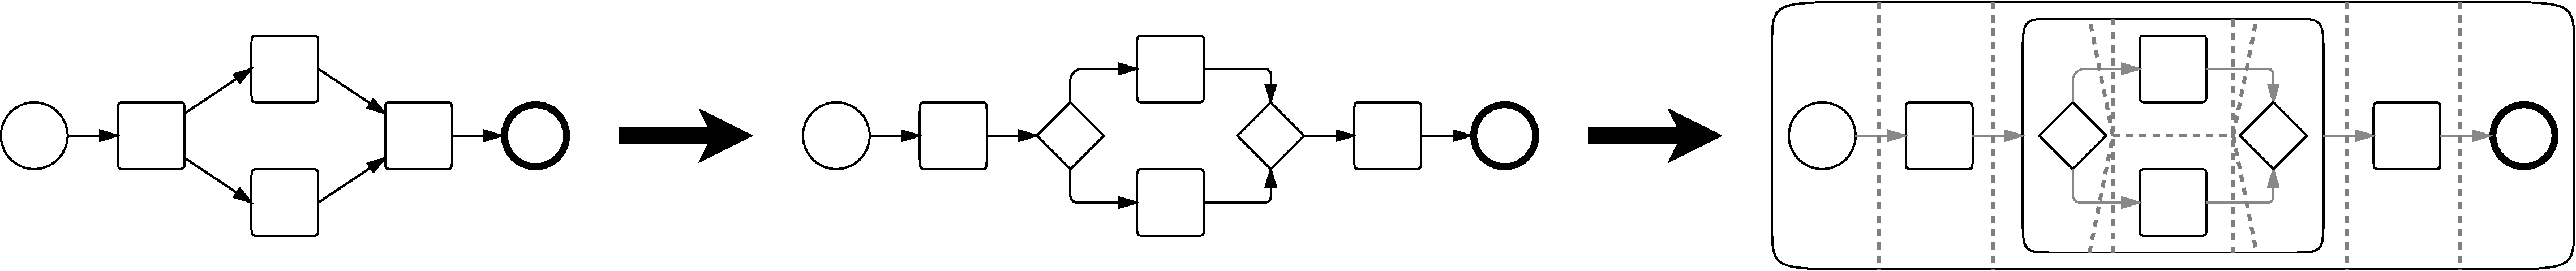
\includegraphics[width=\textwidth]{figures/trafo/norm_struc.pdf}
	\caption{Simple example of normalization and structure mapping.}
	\label{fig:norm_struc}
\end{figure}


\subsection{Transformation of Expressions}

Besides the actual workflow, Expressions that are used in assignments and
conditions have to be translated, too.  This can be done only if the Expression
Language is set to ``VSDT Expression Language'' or ``VXL''.  If then the
\emph{Translate Expressions} option is checked in the Export Wizard (see
Figure~\ref{fig:trafo_wiz}) these expressions will be parsed and, if possible,
translated to the respective target language.

\begin{figure}[ht]
	\centering
	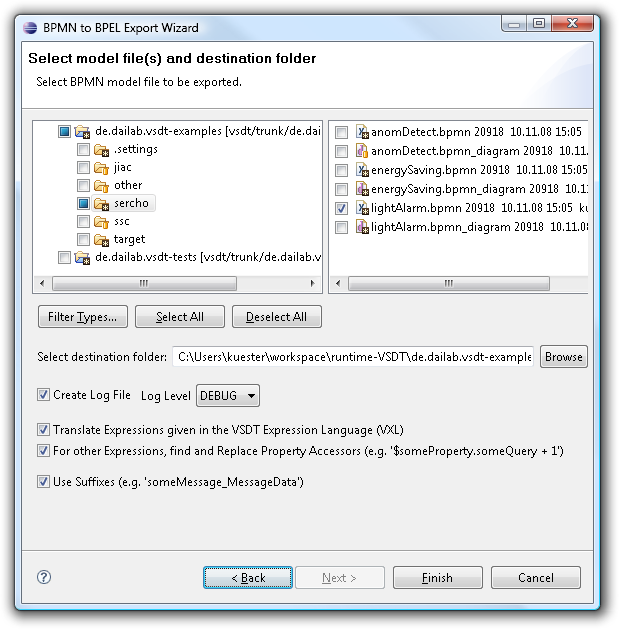
\includegraphics[width=.5\textwidth]{figures/features/exportWiz.png}
	\caption{BPEL Export Wizard with Expression Translation checked.}
	\label{fig:trafo_wiz}
\end{figure}

Still there may be cases when VXL does not have enough expressive power.  In this
case the option can be disabled (or the Expression Language can be changed) and
the \emph{Replace Property Accessors} option can be checked.  Now the Expressions
will only be scanned for Property Accessors in the Form \texttt{\$foo.bar}, which
will then be translated to the syntax of the target language.  Thus, these simple
variable accessors can be embedded in expressions of another language.  For instance,
in the case of BPEL, an expression like \texttt{\$foo.bar + 1}, might be changed
to \texttt{bpws:getVariableData( 'Proc\_ProcessData','foo','bar')+1}.  Thus the
user does not have to care about the way Properties are converted to variables
and how these variables are to be accessed in the transformation to that language
but can simply use a Property's name.

Finally, when Properties are given one of VXL's predefined basic data types (e.g.
\texttt{string}, \texttt{boolean}, etc.), these will be translated to the
respective basic types of the target language, e.g. \texttt{xsd:string} and
\texttt{xsd:boolean}.


%%%%%%%%%%%%%%%%%%%%%%%%%%%%%%%%%%%%%%%%%%%%%%%%%%%%%%%%%%%%%%%%%%%%%%%%%%%%%%%%
%%  Transformation Implementations                                            %%
%%%%%%%%%%%%%%%%%%%%%%%%%%%%%%%%%%%%%%%%%%%%%%%%%%%%%%%%%%%%%%%%%%%%%%%%%%%%%%%%

\section{Transformation Implementations}

The following sections describe in short the various transformations that have
already been implemented.


\subsection{Transformation to Text}

See Section~\ref{sec:user_features_text}.


\subsection{Transformation to BPEL}
\label{sec:user_trafo_bpel}

The transformation to BPEL covers nearly the entire mapping as given in the BPMN
specification~\cite[Appendix A]{omg2011bpmn2}, including event handlers, inclusive
\textsc{or} and event-based \textsc{xor} Gateways, just to name a few.

\paragraph{Export}
Nevertheless there are some elements for which the mapping is not given very
clearly, such as \textsc{timer} Start Events, independent Sub Processes or
multi-instance parallel loops.  While these elements will be transformed as
described in the specification, the resulting BPEL processes will require some
amount of manual refinement.  Besides the BPEL process files a WSDL definitions
file is created, holding the message types derived from the process properties
and the input and output messages and interfaces (port types) for the several Web
services being orchestrated by the process.  Still, the WSDL's binding and service
blocks and necessary schema types, if any, can not be generated automatically
yet, due to insufficient information in the source model.

In the validation, all identifiers are tested to contain only characters that are
legal with respect to BPEL, and all expressions used e.g.\ in assignments and
loop conditions are translated to XPath, if possible.  Properties are aggregated
to one variable per Process or Message; for instance, if a Process \texttt{Proc}
has a Property \texttt{foo}, \texttt{foo} will be a Part of Variable
\texttt{Proc\_ProcessData}.

\paragraph{Import}
The Import from BPEL to BPMN is still at an early stage.  While basic control
flow can be imported, there are still problems e.g. with event- and fault handlers.
Further one should be aware that the export to BPEL does not preserve all
information in the BPMN diagram, thus diagrams re-imported after being exported
to BPEL will most likely be less readable than before, although they may be
semantically equivalent.


\subsection{Transformation to JIAC: JADL++}
\label{sec:user_trafo_jadl}

One of the mayor goals behind the development of the VSDT is the generation of
JIAC multi-agent systems, and specifically JADL services~\cite{kuester2012integrating}.
Note that this work is not yet finished, and thus the mapping of the several
concepts of BPMN and JIAC is still transitional and subject to change.

\paragraph{Export}
A prototypic transformation targeting the agent framework JIAC V has already been
implemented.  In this transformation, the Participants diagram is translated to
an Agent World Diagram~\cite{lutzenberger2009unifying}, and the individual Business
Processes are translated to several JADL services~\cite{hirsch2010programming}.

What's special about the transformation to JIAC is that apart from the JADL
services and the agent configuration, also a set of \emph{service starter rules}
is generated, which can be deployed to a Drools rule engine integrated into the
JIAC agent and which will trigger the different services accordingly to the start
events given in the business process diagrams.


\subsection{Transformation to JIAC: AgentBeans}
\label{sec:user_trafo_agentbeans}

Complementary to the transformation to JIAC V JADL++ Services, also a transformation
to JIAC V Agent Beans~\cite{lutzenberger2013jiacShort} has been implemented~\cite{kuester2014agentbeans}.
While the transformation to JADL is most suitable for high-level services, which
can dynamically be deployed to a running agent platform, the mapping to Agent
Beans is more complete (including event handlers, among others) and more suited
for modeling basic agent behaviors and communication. A formal description of the
mapping is provided by K\"uster et al.~\cite{kuester2015formal}.

\paragraph{Export}
The export to JIAC V Agent Beans covers most parts of the BPMN language,
particularly messaging, event handlers, subprocesses, and process start events.
For each process, one JIAC Agent Bean is created, being made up of one method for
the workflow, and one method for each of the activities.

Similar to the mapping to JADL, also the starting behavior of the processes (the
start events) are mapped to the Agent Beans, but in this case the start event
handling code is integrated into the Bean itself -- no extra Drools rules required.




% \subsection{Transformation to STP-BPMN}
%
% Since BPMN does not provide a standardized interchange format, transferring a
% diagram from one editor to another is difficult.  For that reason the VSDT provides
% a Transformation to the popular Eclipse STP-BPMN Editor.  Thus one can export a
% Diagram to STP-BPMN and carry it to a colleague using that editor, or someone
% formerly using the STP editor can import his existing files when changing to the
% VSDT.
%
% \paragraph{Export}
% The export to STP is nearly complete.  The only elements that are not mapped are
% Lanes, which is because the STP editor is encountering problems when initializing
% the diagram files containing Lanes.  Alas, the same also applies to Embedded
% Subprocesses, as there are problems opening those diagrams.  However, this is a
% problem with the STP editor that will hopefully get fixed soon.
%
% \paragraph{Import}
% The import from STP works very well, with the exception that, again, Lanes will
% not be mapped. \emph{Note} that the transformation to STP will only create the
% BPMN model files, but not the diagram files; those files, holding the graphical
% information, have to be generated anew from the model file.  Consequently, the
% transformation does not preserve the layout of the diagrams.
%
% The \emph{BPMN to STP-BPMN Transformation} feature requires the \emph{Eclipse SOA
% Tools Project BPMN Editor} feature.


%%%%%%%%%%%%%%%%%%%%%%%%%%%%%%%%%%%%%%%%%%%%%%%%%%%%%%%%%%%%%%%%%%%%%%%%%%%%%%%%
%%  Limitations                                                               %%
%%%%%%%%%%%%%%%%%%%%%%%%%%%%%%%%%%%%%%%%%%%%%%%%%%%%%%%%%%%%%%%%%%%%%%%%%%%%%%%%

\section{Limitations}

Although the transformation framework is quite powerful, it is important to
understand that there are still some limitations, both in the mapping of
structures and of elements.

\begin{itemize}
	\item Given a well-structured workflow, the transformation yields very good
	results.  However, as BPMN is more expressive that block-oriented languages,
	such as BPEL and JIAC, there will always be graph structures that can not be
	transformed to an equivalent program of the target language.  In that case
	the diagram should be manually restructured \emph{before} being exported.

	\item The mapping to BPEL is as complete as possible, according to the
	specification.  Still, there are some points in the specification that are
	missing, unclear or ambiguous.  The transformation to BPEL is implementing
	the specification in almost every detail, but regarding these elements a small
	amount of manual refinement may be necessary.

	\item The mapping to JADL++ is still at an early stage.  For a subset of both
	BPMN and JADL, the transformation yields good results and can be used for
	creating meaningful, executable scripts, but there are still some open issues.
\end{itemize}

We are constantly investigating ways of extending both the quality of the element
mappings and the performance of the structure mapping.

